% Template for PLoS
% Version 3.1 February 2015
%
% To compile to pdf, run:
% latex plos.template
% bibtex plos.template
% latex plos.template
% latex plos.template
% dvipdf plos.template
%
% % % % % % % % % % % % % % % % % % % % % %
%
% -- IMPORTANT NOTE
%
% This template contains comments intended 
% to minimize problems and delays during our production 
% process. Please follow the template instructions
% whenever possible.
%
% % % % % % % % % % % % % % % % % % % % % % % 
%
% Once your paper is accepted for publication, 
% PLEASE REMOVE ALL TRACKED CHANGES in this file and leave only
% the final text of your manuscript.
%
% There are no restrictions on package use within the LaTeX files except that 
% no packages listed in the template may be deleted.
%
% Please do not include colors or graphics in the text.
%
% Please do not create a heading level below \subsection. For 3rd level headings, use \paragraph{}.
%
% % % % % % % % % % % % % % % % % % % % % % %
%
% -- FIGURES AND TABLES
%
% Please include tables/figure captions directly after the paragraph where they are first cited in the text.
%
% DO NOT INCLUDE GRAPHICS IN YOUR MANUSCRIPT
% - Figures should be uploaded separately from your manuscript file. 
% - Figures generated using LaTeX should be extracted and removed from the PDF before submission. 
% - Figures containing multiple panels/subfigures must be combined into one image file before submission.
% For figure citations, please use "Fig." instead of "Figure".
% See http://www.plosone.org/static/figureGuidelines for PLOS figure guidelines.
%
% Tables should be cell-based and may not contain:
% - tabs/spacing/line breaks within cells to alter layout or alignment
% - vertically-merged cells (no tabular environments within tabular environments, do not use \multirow)
% - colors, shading, or graphic objects
% See http://www.plosone.org/static/figureGuidelines#tables for table guidelines.
%
% For tables that exceed the width of the text column, use the adjustwidth environment as illustrated in the example table in text below.
%
% % % % % % % % % % % % % % % % % % % % % % % %
%
% -- EQUATIONS, MATH SYMBOLS, SUBSCRIPTS, AND SUPERSCRIPTS
%
% IMPORTANT
% Below are a few tips to help format your equations and other special characters according to our specifications. For more tips to help reduce the possibility of formatting errors during conversion, please see our LaTeX guidelines at http://www.plosone.org/static/latexGuidelines
%
% Please be sure to include all portions of an equation in the math environment.
%
% Do not include text that is not math in the math environment. For example, CO2 will be CO\textsubscript{2}.
%
% Please add line breaks to long display equations when possible in order to fit size of the column. 
%
% For inline equations, please do not include punctuation (commas, etc) within the math environment unless this is part of the equation.
%
% % % % % % % % % % % % % % % % % % % % % % % % 
%
% Please contact latex@plos.org with any questions.
%
% % % % % % % % % % % % % % % % % % % % % % % %

\documentclass[10pt,letterpaper]{article}
\usepackage[top=0.85in,left=2.75in,footskip=0.75in]{geometry}

% Use adjustwidth environment to exceed column width (see example table in text)
\usepackage{changepage}

% Use Unicode characters when possible
\usepackage[utf8]{inputenc}

% textcomp package and marvosym package for additional characters
\usepackage{textcomp,marvosym}

% fixltx2e package for \textsubscript
\usepackage{fixltx2e}

% amsmath and amssymb packages, useful for mathematical formulas and symbols
\usepackage{amsmath,amssymb}

% cite package, to clean up citations in the main text. Do not remove.
\usepackage{cite}

% Use nameref to cite supporting information files (see Supporting Information section for more info)
\usepackage{nameref,hyperref}

% line numbers
\usepackage[right]{lineno}

% ligatures disabled
\usepackage{microtype}
\DisableLigatures[f]{encoding = *, family = * }

% rotating package for sideways tables
\usepackage{rotating}

% Remove comment for double spacing
%\usepackage{setspace} 
%\doublespacing

% Text layout
\raggedright
\setlength{\parindent}{0.5cm}
\textwidth 5.25in 
\textheight 8.75in

% Bold the 'Figure #' in the caption and separate it from the title/caption with a period
% Captions will be left justified
\usepackage[aboveskip=1pt,labelfont=bf,labelsep=period,justification=raggedright,singlelinecheck=off]{caption}

% Use the PLoS provided BiBTeX style
\bibliographystyle{plos2015}

%%%%%%%%%%%%%%%%%%%%%%% START - MY SETUP %%%%%%%%%%%%%%%%%%%%%%%%%%%%%%

\usepackage{url}\urlstyle{same}
\usepackage{booktabs}
\usepackage{colortbl, xcolor}
\usepackage{epstopdf}
\usepackage{array}
\setlength\extrarowheight{2pt}

% rysunki
\usepackage{tikz}
\usepackage{ifthen}
\usepackage{xxcolor}
\usetikzlibrary{arrows}
\usetikzlibrary[topaths]
\usetikzlibrary{decorations.pathreplacing}

%%%%%%%%%%%%%%%%%%%%%%% END - MY SETUP %%%%%%%%%%%%%%%%%%%%%%%%%%%%%%

% Remove brackets from numbering in List of References
\makeatletter
\renewcommand{\@biblabel}[1]{\quad#1.}
\makeatother

% Leave date blank
\date{}

% Header and Footer with logo
\usepackage{lastpage,fancyhdr,graphicx}
\usepackage{epstopdf}
\pagestyle{myheadings}
\pagestyle{fancy}
\fancyhf{}
\lhead{
\includegraphics[width=2.0in]{PLOS-submission.eps}}
\rfoot{\thepage/\pageref{LastPage}}
\renewcommand{\footrule}{\hrule height 2pt \vspace{2mm}}
\fancyheadoffset[L]{2.25in}
\fancyfootoffset[L]{2.25in}
\lfoot{\sf PLOS}

%% Include all macros below

\newcommand{\lorem}{{\bf LOREM}}
\newcommand{\ipsum}{{\bf IPSUM}}

\newcommand{\beginsupplement}{%
        \setcounter{subsection}{0}
        \renewcommand{\thesubsection}{S\arabic{subsection}}
     }

%% END MACROS SECTION


\begin{document}
\vspace*{0.35in}

% Title must be 250 characters or less.
% Please capitalize all terms in the title except conjunctions, prepositions, and articles.
\begin{flushleft}
{\Large
\textbf\newline{Prediction of signal peptides in proteins from malaria parasites}
}
\newline
% Insert author names, affiliations and corresponding author email (do not include titles, positions, or degrees).
\\
Micha\l{}  Burdukiewicz\textsuperscript{1},
Piotr Sobczyk\textsuperscript{2},
Pawe\l{} B\l{}a\.{z}ej\textsuperscript{1},
Pawe\l{} Mackiewicz*\textsuperscript{1},
\\
\bigskip
\bf{1} University of Wroc\l{}aw, Department of Genomics, Poland
\\
\bf{2} Wroc\l{}aw University of Technology, Department of Mathematics, Poland
\\
\bigskip

% Use the asterisk to denote corresponding authorship and provide email address in note below.
* pamac@smorfland.uni.wroc.pl

\end{flushleft}
% Please keep the abstract below 300 words
\section*{Abstract}
Signal peptides play an essential role in targeting substantial number of proteins to endomembrane system and their export outside the cell. Such proteins are of great importance in metabolism, maintenance of tissue structure, immune response and regulation of other organismal functions. The software for computional recognition of these peptides usually employs learning systems. To make correct predictions, these algorithms require big data sets consisting of signal peptides from different types of proteins and taxonomic groups. Therefore, they perform well in general identification of typical signal peptides but are ineffective in atypical ones, for which it is not possible to obtain sufficiently large data sets for  learning algorithms. Such class of peptides is present in many proteins from parasites belonging to the phylum Apicomplexa. Their members, especially \textit{Plasmodium}, are of great medically significance being a malaria agent. That is why, we designed a new more flexible probabilistic model for recognition of eukaryotic signal peptides, which includes knowledge about their organization, amino acid composition and variability. The proposed approach called signalHsmm is based on hidden semi-Markov models (HSMMs). It is able to recognize signal peptides from the malaria parasites and their relatives more accurately (with AUC = 0.94) than popular programs (0.89), still being universal enough to provide prediction of other eukaryotic signal peptides on par with the best preforming predictors. Moreover, it proves to be very stable regardless of type of learning data. Therefore, our model does not need to be permanently retrained with the continuous expansion of sequence databases. The web-server of signalHsmm is available at \url{http://smorfland.uni.wroc.pl/signalhsmm}.


% Please keep the Author Summary between 150 and 200 words
% Use first person. PLOS ONE authors please skip this step. 
% Author Summary not valid for PLOS ONE submissions.   
%\section*{Author Summary}


\linenumbers

\section*{Introduction}
\subsection*{Roles and features of signal peptides}

Proteins of eukaryotes are encoded in nuclear genomes and are synthesized in ribosomes located in the cytosol or bounded by the endoplasmic reticulum. After translation, proteins are targeted to specific subcellular compartments or exported outside the cell. The proper localization of proteins is essential to perform their desired function. Information about the protein destination is included within the very protein in short stretches of amino acid residues called targeting or sorting signals. One kind of them are signal peptides, which are located at the N-terminus of proteins.

Signal peptides are responsible for targeting of proteins via the Sec61 translocation channel~\cite{2007rapoportprotein} to endomembrane system, which includes endoplasmic reticulum and Golgi apparatus. Such proteins can stay inside these compartments, can be inserted into cellular membranes or exported outside the cell. Proteins equipped with signal peptides play crucial role in metabolism ($\beta$-galactosidase, pepsins)~\cite{1991hofmannmutations}, maintenance of tissue structure (collagen)~\cite{2001chanaberrant}, immune response (interferons, interleukins)~\cite{2005zhangalteration} and regulation of other organismal functions (prolactin, glucagon)~\cite{2010huangrole}. Moreover, passing proteins through the endomembrane system is important for their correct folding and posttranslational modification such as glycosylation and phosphorylation.

Despite the low sequence homology between signal peptides~\cite{1999ladungaphysean}, some general architecture was proposed~\cite{1994izardsignal, 2013vossmechanism} - Fig. \ref{fig:sparch}. It is assumed that signal peptides start with a positively charged sequence of amino acid residues, called the n-region with the length of about 5-8 residues. They probably enforce a proper topology on a polypeptide during its translocation through the membrane based on the positive-inside rule~\cite{1988vonheijnetopogenic}. The first region is followed by a stretch of hydrophobic amino acids (h-region) with the length of about 8-12 residues. It constitutes a core region of signal peptide and usually forms $\alpha$-helix. The third part of a signal peptide is a polar and uncharged c-region. It is usually 6 residues long and ends with a cleavage site, in which a signal peptidase cleaves the signal peptide, during or after translocation of the protein into the lumen of endoplasmic reticulum ~\cite{2002paetzelsignal}. The cleavage site is characterized by a variable amino acid composition. It typically contains small and neutral residues at -3 and -1 positions~\cite{1994palzkillselection}. This site is, however, absent from some membrane proteins in which the first transmembrane domain acts both as a signal peptide and signal anchor~\cite{1988szczesnaskorupapositive}. The amino acid composition and the length of these regions vary between signal peptides, which influences the efficiency of protein secretion~\cite{2006hegdethe}.

\begin{figure}[ht]\centering
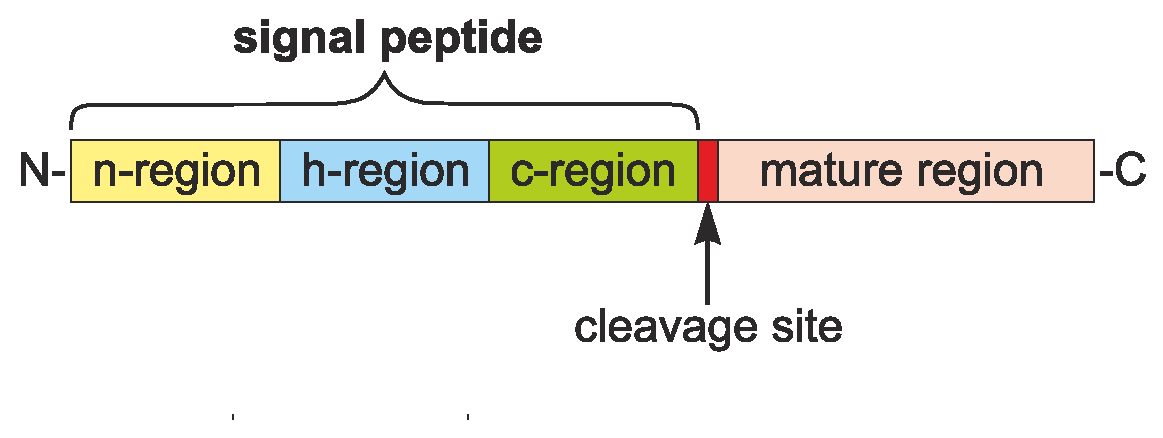
\includegraphics[width=0.55\textwidth]{figures/SP.eps}
\caption{The organization of typical signal peptide. The regions are not drawn in scale.}
\label{fig:sparch}
\end{figure}

On the other hand, signal peptides show a great variation and the description presented above (Fig. \ref{fig:sparch}) refers to the most "typical" signal peptides. There are  exceptionally long signal peptides, which fulfill more sophisticated roles~\cite{2009hissarchitecture}. For example, the fragment of signal peptide from preprolactin takes part in the regulation of prolactin secretion, whereas signal peptides of MHC class I inhibit activity of NK cells. Signal peptides of viral origin are involved in the immune evasion or viral life cycle~\cite{2000kappposttargeting} and the signal peptide from midkine, containing epitopes recognized by CD4+ T cells, contributes to tumor progression ~\cite{2013kerzerhothe}. 

The functional significance of these targeting signals makes that the prediction of signal peptide-containing proteins is an important step in the drug development~\cite{2005zhangalteration, 2012netoadeimproving, 2010moellerwetmilling}. The signal peptides can be  potential drug targets, especially for malaria parasites from the genus \textit{Plasmodium} belonging to the phylum Apicomplexa. Their signal peptides not only direct proteins into endomembrane system or outside the cell but also into a unique organellum specific only for \textit{Apicomplexa}, called apicoplast~\cite{2003foththe, Lim2010, McFadden, Heiny2014}. It is a reduced four-membrane plastid, which lost photosynthetic function but play an important role in synthesis of fatty acids and lipids~\cite{Lim2010, McFadden, Mazumdar2006}. Therefore, anti-malarial drugs disturbing pathways targeting proteins into the apicoplast should be safe for human (host) and harmful for the parasite~\cite{1997ficheraa, ralph, 2003gornickiapicoplast, 2010garciaestradadna}. Other potential apicomplexan drug target, the food vacuole, also imports proteins tagged with the signal peptide~\cite{2002egandiscovering}. A model of \textit{Plasmodium} signal peptide would aid in the design of appropriate medicines. However, the targeting signals of \textit{Plasmodium} proteins show deviated composition in comparison to typical signals because of heavy adenine-thymine bias of parasitic genomes~\cite{Tonkin2008a}. Therefore, the current programs dedicated to recognition of general eukaryotic signal peptides are not appropriate.


\subsection*{Software predicting signal peptides}

Since experimental methods determining the subcellular localization of proteins and identifying signal peptide are time-consuming and laborious, different computational approaches predicting targeting signals were developed. Among them, signal peptides became the subject of several computational programs to their prediction. Many software incorporates 'black-box’ models, such as: neural networks~\cite{2011petersensignalp}, support vector machines~\cite{2014zhangprediction}, Bayesian networks~\cite{2012zhengsignalbnf} or k-nearest neighbours~\cite{2007shensignall}. However, these models do not provide direct biological information about organization of signal peptides and are not able to predict properly atypical signal peptides. Although there are programs that do not share the innate flaws of 'black-box' models, they also demand an improvement. Some of them are based on position matrices or their variants~\cite{2014zhangprediction, 2004hillerpredisi}. Others (Phobius, Philius and SignalP 3.0) use hidden Markov models (HMMs)~\cite{2004klla, 2008reynoldstransmembrane, 2004bendtsenimproved}, which try to reflect structure of signal peptides regions in their limited probabilistic frameworks. The used HMMs, however, imply a geometric distribution for duration of regions length. We studied the distribution for regions from the first work utilizing HMMs in prediction of signal peptides~\cite{1998nielsenprediction} and found that the length distribution for every region was not geometric (Fig. \ref{fig:reglen}).

Majority of the signal peptide predicting software uses the orthogonal encoding of amino acids, in which a vector of 20 digits represents every amino acid. This method of encoding, however, does not take into account relationships between amino acids and differences in their physicochemical properties. This is disadvantage of such signal peptide's models because their regions are in fact characterized by specific features of amino acid residues and not by the simple occurrence of particular amino acids. In addition to this, such sparse encoding requires large data sets, which hinders their management and analysis~\cite{2002linamino}. 

Moreover, the present algorithms require the big number of sequences to be successfully learned. That is why, such sets consists of peptides coming from different types of proteins and taxonomic groups. As a result of this, they perform well in general identification of typical signal peptides but are ineffective in atypical ones, for which it is not possible to obtain sufficiently large data sets to effectively learn recognizing algorithms. The commonly used rigid scheme of signal peptide's organization (Fig. \ref{fig:sparch}) does not characterize extremely long or short peptides, which constitute substantial fraction of all signal peptides. Theoretically, HMMs that describe the atypical signal peptides could be developed to consider also the unusual structures but such probabilistic frameworks have not yet been implemented. Therefore, we elaborated a new approach called signalHsmm based on hidden semi-Markov models using grouping of amino acids into physicochemical groups characteristic of signal peptides. The recent advancements in the proteomics suggest that such simplification of amino acid alphabet (by reducing the number of letters) may lead to better fold recognition~\cite{2000murphysimplified, 2009petersonreduced}. Considering that one of key features of signal peptide is its secondary structure ($\alpha$-helix), the universal model may utilize shorter amino acid alphabet, where several similar amino acids are unified into a single group. It enabled us to design a new more flexible probabilistic model for recognition of eukaryotic signal peptides including atypical peptides in \textsl{Plasmodium}.



\begin{figure}[ht]\centering
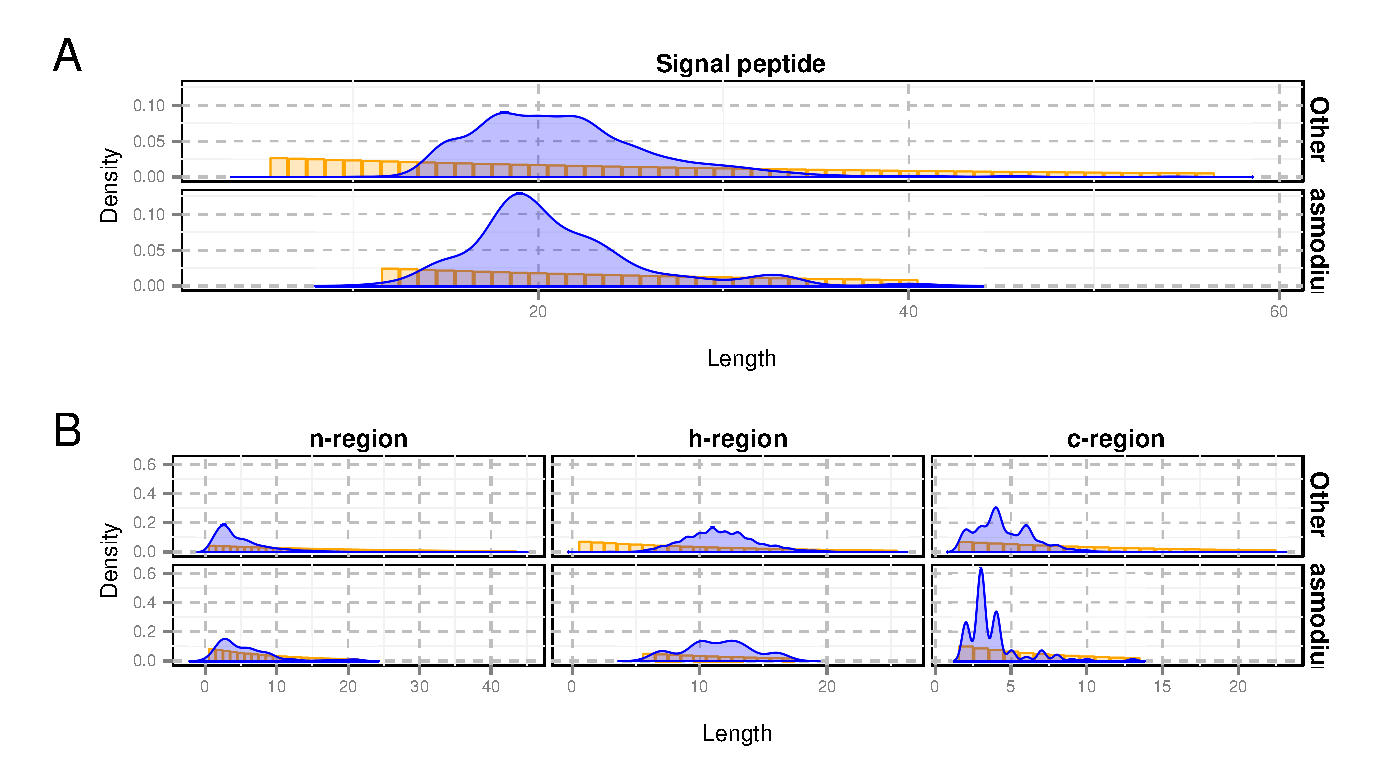
\includegraphics[width=0.95\textwidth]{figures/reglen.eps}
\caption{Distribution of lengths for signal peptides (A) and their regions (B) expressed in the number of amino acid residues for sequences excluding members of \textit{Plasmodiidae} family (Other) and members of this family (Plasmodium). Yellow bars represent a fitted geometric distribution.}
\label{fig:reglen}
\end{figure}

% All programs used in signal peptide recognition are trained on real protein sequences. Therefore, they succeed in the recognition of peptides similar to those in the learning set but fail in the case of artificial signal peptides. Such peptides are designed to increase effectiveness of protein secretion~\cite{2010futatsumorisugaisignal}. They are especially important in industrial applications to increase yield of proteins. Therefore, only explicit knowledge about the organization of signal peptides allows creating sequences that will be the most efficient in the export of proteins~\cite{2013ngengineering}. Signal peptides have also an important application in gene therapy. Mimicking the natural mechanism of protein export, artificial signal peptides with tumor epitopes increase the antitumor immune response~\cite{2003heenhanced}. Such epitopes must be properly inserted into a signal peptide without decreasing its secretion properties through disruption of the regional structure. Instead of time-consuming and expensive laboratory experiments, it would be very useful to survey \textit{in silico} many artificial peptides to select the ones that would fulfill the designed role.



\section*{Materials and Methods}

\subsection*{Overview}

Since the functionality of signal peptides depends on the physicochemical properties of residues in a given region, we clustered amino acids into several groups based on their features. The pre-processed sequences were further analyzed by an heuristic algorithm, which determines borders between three characteristic regions in signal peptides, which is an enhanced version of heuristic algorithm employed in signalP 2.0~\cite{1998nielsenprediction}. We refined some criteria in recognition of the regions to attune the algorithm to less typical signal peptides. Next, two models were trained to recognize proteins with and without a signal peptide. The first one was a hidden semi-Markov model, in which each of three signal peptide's regions was represented by a different hidden state. The additional fourth hidden state represented a mature protein. Each state was described by its frequencies of amino acid groups. The distribution of hidden states durations, i.e. the number of amino acids, was based on the empirical distribution of region lengths from the training set. Furthermore, the hidden semi-Markov model was enriched with n-grams representing signal peptide cleavage sites. The second model was a simple probabilistic approach in which no association between amino acids was assumed and probability of amino acids groups occurrence was determined by their frequencies in mature proteins.

\subsection*{Data selection}

The final predictor was trained on 2438 experimentally confirmed signal peptides from eukaryotic proteins, whose sequences and annotations were downloaded from UniProt database release 2015\_06. We removed sequences with more than one cleavage site, unknown cleavage site and ambiguous symbols of amino acid residues: X, J, Z, B and U (selenocysteine). Sequences without signal peptide were randomly selected in the same number as the positive set. Moreover, we created a learning subset of sequences deposited in the database till 2010 year to performed honest comparison of our algorithm with older software trained on smaller number of sequences. We also used a subset of sequences present in the database till 1987 year, just after the first method predicting signal peptide was published, to check susceptibility of our algorithm to limited amount of information (Tab.~\ref{tab:sets}).

The main testing set consisting of proteins belonging to the organisms from \textit{Plasmodiidae} family. The positive set contained 102 sequences with a putative signal peptide having annotated start and cleavage site. The corresponding negative set comprised 358 sequences without any signal peptide information. The other testing set consists of 127 eukaryotic proteins with signal peptide included in the UniProt database after 2010 year. 

 
\subsection*{Homology reduction of studied sequence sets}

To reduce the set according to homology of collected protein sequences, we filtered them using cd-hit~\cite{2012fucdhit}. The homology reduction were subjected sequences of signal peptides and the first 70 amino acid residues in the case of proteins without the peptide, as proposed by~\cite{1997nielsenidentification}. We prepared two learning data sets by removing the homology on 50\%-similarity threshold with word length 2 (Tab.~\ref{tab:sets}). The testing set was filtered in the same manner. After this procedure, these sets were reduced to 51 and 211 sequences with and without signal peptide, respectively.


\begin{table}[ht]
\centering
\caption{Number of sequences with signal peptides used in the study for  different types of learning sets.} 
\label{tab:sets}
\begin{tabular}{ccc}
  \toprule
		\multirow{Set} &
		\multicolumn{2}{c}{Homology reduction}\\
		\cline{2-3}
 & No & 50\% \\ 
  \midrule
\rowcolor[gray]{0.85}Till 2015 & 2438 & \\ 
   Till 2010 & 2311 & 748 \\ 
  \rowcolor[gray]{0.85}Till 1987 & 336 & 132 \\ 
   \bottomrule
\end{tabular}
\end{table}



\subsection*{Clustering of amino acids into groups}

To reduce alphabet of amino acids, we clustered them into several physico-chemical groups. It is a different approach in comparison to BLOMAP~\cite{maetschke2005blomap}, which also uses a reduced alphabet of amino acids but based on substitution matrices. We grouped amino acids using four properties relevant for the architecture of signal peptide: their hydrophobicity, tendency to occurring in  $\alpha$-helices, polarity and size. The high hydrophobicity is a good determinant of the h-region, whose $\alpha$-helix secondary structure is probably induced by the positively charged n-region. The high polarity as well as small size are important features of residues in the c-region and cleavage site~\cite{1994palzkillselection}.

\begin{table}[ht]
\centering
\caption{Properties of amino acids used in their clusterization.} 
\begin{tabular}{ll}
  \toprule
Property name & Amino acid scale \\ 
  \midrule
Size & Size~\cite{dawson1972size} \\ 
   \rowcolor[gray]{0.85}Size & Molecular weight~\cite{fasman1976handbook}\\ 
  Size & Residue volume~\cite{1973goldsackcontribution} \\ 
   \rowcolor[gray]{0.85}Size & Bulkiness~\cite{1968zimmermanthe} \\ 
  Hydrophobicity & Normalized hydrophobicity scales for $\alpha$-proteins~\cite{1992cidhydrophobicity} \\ 
   \rowcolor[gray]{0.85}Hydrophobicity & Consensus normalized hydrophobicity scale~\cite{1984eisenbergthreedimensional} \\ 
  Hydrophobicity & Hydropathy index~\cite{1982kytea} \\ 
   \rowcolor[gray]{0.85}Hydrophobicity & Surrounding hydrophobicity in $\alpha$-helix~\cite{1980ponnuswamyhydrophobic} \\ 
  Polarity & Polarity~\cite{1974granthamamino} \\ 
   \rowcolor[gray]{0.85}Polarity & Mean polarity~\cite{1988radzickainfluences} \\ 
  Occurrence in $\alpha$-helices & Signal sequence helical potential~\cite{1982argosstructural} \\ 
   \rowcolor[gray]{0.85}Occurrence in $\alpha$-helices & Normalized frequency of N-terminal helix~\cite{chou1978prediction} \\ 
  Occurrence in $\alpha$-helices & Relative frequency in $\alpha$-helix~\cite{1990prabhakaranthe} \\ 
   \bottomrule
\end{tabular}
\label{tab:aaprop}
\end{table}

We considered in total 13 amino acid scales present in AAIndex database~\cite{2008kawashimaaaindex} (Tab.~\ref{tab:aaprop}). We selected one scale per a given property and carried out all possible 96 permutations of them. Based on that, we created 96 possible clusterings of amino acids using Euclidean distance and Ward's method. Next, we cut the clusterings to create four group of amino acids. In 31\% of cases, the groupings were identical. To compare the usefulness of these encodings, we performed a 5-fold cross-validation training our algorithm on every encoding. We created balanced data sets by subsampling proteins without a signal peptide to equal the number of proteins with a signal peptide. The cross-validation was repeated 60 times to ensure that every protein without signal peptide was included in the learning set with the probability higher than 0.5.

\subsection*{Hidden semi-Markov model}
Our algorithm is based on hidden semi-Markov model (HSMM), which is an extension of hidden Markov model (HMM)~\cite{1989rabinera, Yu2010215, koski_hidden_2001}. The HMM consists of two stochastic processes. The first is a discrete Markov chain $X_{t=1}^T$ on the set of  hidden states $\{S_1, \dots S_n\}$, where $t$ means a step of this process and $T$ means the total duration of the process corresponding to the length of signal peptide. The hidden states represent particular signal peptide regions and are "the cause" of the observations, which are amino acid residues in analyzed sequences. In a subsequent step $t+1$, the hidden state might change to another according to a transition matrix $A = (a)_{i,j=1}^n$, where $a_{i,j} = \mathcal{P}(X_{t+1} = S_j | X_t = S_i)$ means a probability of being in a state $j$ on condition that in the previous step was a state $i$. The second process $E_{t=1}^T$ is an observation process defined on the set of possible observations $\{O_1, \dots, O_m\}$. They are assumed to occur independently but conditionally on the hidden states that emits these observations. 
The distribution of observations are given by a matrix $B = (b)_{i,k=1}^m$, where $b_{i,k} = \mathcal{P}(E_t = O_k | X_t = S_i)$ means a probability of emission of observation $k$ on condition that a hidden state was $i$.
The main goal of signalHsmm is to find the most probable signal peptide's regions boundaries for a given sequences. This is achieved with Viterbi algorithm.

In the regular HMM, the hidden state duration, i.e. the number of observations emitted by the hidden state, has a geometric distribution. Durbin et al.~\cite{Durbin98} showed how to extend it for different distributions without significant increase in computational 
complexity. Similar ideas were used for signal peptide recognition, for example by~\cite{2004klla}. However, it is still not flexible enough because the empirical regional length distributions (see Fig.~\ref{fig:reglen}) are difficult to capture in this way.

%rysunek pokazujący o co chodzi w HMM
\begin{figure}[h]
\centering
\tikzstyle{block} = [draw,shape=circle, top color=green!50!white!70, bottom color=green!50!white!70 ,minimum size=4em]
\tikzstyle{blockComp} = [draw,shape=circle, top color=red!50!white!70, bottom color=red!50!white!70 ,minimum size=2.5em]
% diameter of semicircle used to indicate that two lines are not connected
\def\radius{.7mm} 
\tikzstyle{branch}=[shape=rectangle, top color=white, bottom color=white ,minimum size=3pt,inner sep=0pt]
\tikzstyle{branch2}=[shape=rectangle, top color=white, bottom color=white ,minimum size=3pt,inner sep=0pt]
\def\n{11}
 \tikzstyle{line} = [draw=black, color=black!70!white!50, line width=1.5mm, -latex'] 
 \tikzstyle{line2} = [draw=black, color=red!30!white!70, line width=1.5mm, -latex']
\tikzstyle{frame}=[text=black,above, bottom color=white, top color=blue!50!black!70  ]
\tikzstyle{frameComp}=[text=black,below, bottom color=red!50!white!70, top color=red!50!white!70  ]
 \tikzstyle{line3} = [color=green!50!black!70, line width=1.5mm]
\def\names{{"$O_{1,1}$","...","$O_{1,d_1}$", "...","$O_{n, 1}$", "...", "$O_{n, d_n}$"}}%
\begin{tikzpicture}[>=latex']
%wąsate nawiasy
%\draw [decorate, decoration={brace,amplitude=10pt},line3,xshift=0pt,yshift=0pt] (2.5,1) -> (10.5,1) node [branch,midway,yshift=0.8cm,color=black] 
	%{\textbf{Hidden states}};
% \draw [->,decoration={brace,mirror,amplitude=10pt},line2,xshift=0pt,yshift=0pt] (11,-3) -- (3,-3) node [branch2,midway,yshift=-0.6cm,color=black] 
% 	{\textbf{Kierunek odczytu na nici Cricka ($3' \to 5'$)}}; 
   % Draw blocks, inputs and outputs
 
\node[block] at (1+2,0) (block1) {\footnotesize $S_1$};
\node[blockComp] at (-.5+2,-2)  (komp1) {\footnotesize \pgfmathparse{\names[0]}\pgfmathresult};
\node[blockComp] at (1+2,-2)  (komp2) {\footnotesize \pgfmathparse{\names[1]}\pgfmathresult};
\node[blockComp] at (2.5+2,-2)  (komp3) {\footnotesize \pgfmathparse{\names[2]}\pgfmathresult};
\draw[line,->]  (block1) --  (komp1);
\draw[line,->]  (block1) --  (komp2);
\draw[line,->]  (block1) --  (komp3);
\draw[line3,->] (block1.east) -- +(2,0) node [branch,midway,yshift=0.3cm,xshift=-0.2cm,color=black] {\footnotesize \textbf{transition}};

\node[block, bottom color=green!50!white!80,] at (4.5+2,0) (block2) {...};
\draw[line3,->] (block2.east) -- +(2,0) node [branch,midway,yshift=0.3cm,xshift=-0.2cm,color=black] {\footnotesize \textbf{transition}};
\node[blockComp] at (4.5+2,-2)  (komp4) {\footnotesize \pgfmathparse{\names[3]}\pgfmathresult};
\draw[line,->]  (block2) --  (komp4) ;

\node[block, bottom color=green!50!white!70] at (8+2,0) (block3) {\footnotesize $S_n$};
\node[blockComp] at (6.5+2,-2)  (komp5) {\footnotesize \pgfmathparse{\names[4]}\pgfmathresult};
\node[blockComp] at (8+2,-2)  (komp6) {\footnotesize \pgfmathparse{\names[5]}\pgfmathresult};
\node[blockComp] at (9.5+2,-2)  (komp7) {\footnotesize \pgfmathparse{\names[6]}\pgfmathresult};
\draw[line,->]  (block3) --  (komp5);
\draw[line,->]  (block3) --  (komp6);
\draw[line,->]  (block3) --  (komp7);

% \draw[<->, color=red!30!black!50, line width=1.5mm] (komp1) |- +(5,-1.5) node[line2, yshift=-0.5cm] {\textbf{Observations}} -| (komp7); 

\draw [color=red!50!black!70, line width=1.5mm, decorate,decoration={brace,amplitude=10pt,mirror,raise=10pt},yshift=-10pt]
(1,-1.8) -- (5,-1.8) node [branch2, midway, yshift=-1cm,color=black] {\textbf{Duration of length $d_1$}};

\draw [color=red!50!black!70, line width=1.5mm, decorate,decoration={brace,amplitude=10pt,mirror,raise=10pt},yshift=-10pt]
(8,-1.8) -- (12,-1.8) node [branch2, midway, yshift=-1cm,color=black] {\textbf{Duration of length $d_n$}};

\draw [color=red!50!black!70, line width=1.5mm, decorate,decoration={brace,amplitude=15pt,mirror,raise=10pt},yshift=-10pt]
(1,-2.6) -- (12,-2.6) node [branch2, midway, yshift=-1.3cm,color=black] {\textbf{Total duration, $\sum_{i=1}^k d_i = T$}};
\end{tikzpicture}
\caption{General scheme of hidden semi-Markov model. The model consists of hidden states $S$ representing regions of a signal peptide with the length distribution given by the state duration $d$. The hidden states emit observations $O$ which are amino acid residues.}
\label{fig:hsmm}
\end{figure}

In our approach, we used a modification of HMM called hidden semi-Markov model (HSMM)~\cite{Yu2010215}. It extends the HMM by assuming a duration distribution for a given hidden state (Fig.~\ref{fig:hsmm}). Then, the model includes additionally probabilities of duration in hidden states: 
$$\mathcal{P}(\text{duration in state} = d | \text{state is } S_i), \;\; i = 1, \dots, n, \;\; d = 1, \dots, D$$,
where $D$ is the maximum allowed duration.
Since our data sets are sufficiently large and $D$ is small -- around 30 amino acid residues, computational effort is not much higher than in the regular HMM. 

Almost all entries in the transition matrix $A$ are zeros because regions represented by hidden states are sequential. Possible transitions between them are depicted as arrows in Fig.~\ref{fig:ngramext}. Probabilities of observations for the hidden states and hidden states durations were estimated from training data. The advantage of HSMM model results not only from its better performance but also form its straightforwardness and flexibility. 


%model structure

\begin{figure}[ht]\centering

\includegraphics[width=0.51\textwidth]{figures/HSMMs.eps}
\caption{The diagram of simple (A) and extended version of signalHsmm with the n-gram cleavage site model (B).}
\label{fig:ngramext}
\end{figure}

    
% \subsection*{Extension of n-grams}
% 
% Hidden semi-Markov models can be easy enhanced by inclusion of additional hidden states. To improve our model, we added few supplementary states representing specific motives that can occur in the proximity of cleavage site. The sequence of cleavage sites is more conserved than other parts of signal peptide~\cite{2004hillerpredisi} and can be described by n-grams (k-mers, short vectors of $n$ characters derived from input sequences). Using the biogram software~\cite{biogramPackage}, we extracted n-grams from cleavage sites of signal peptides. Their sequences were encoded using amino acid classification providing the best sensitivity of the general model (Tab. \ref{tab:best}). Selected n-grams representing less common cleavage site motifs were included in the HSMM model as alternative paths at the end of c-region (Fig.~\ref{fig:ngramext}B).


\section*{Results and discussion}

\subsection*{Performance of signalHsmm algorithm}

\begin{figure}[ht]\centering
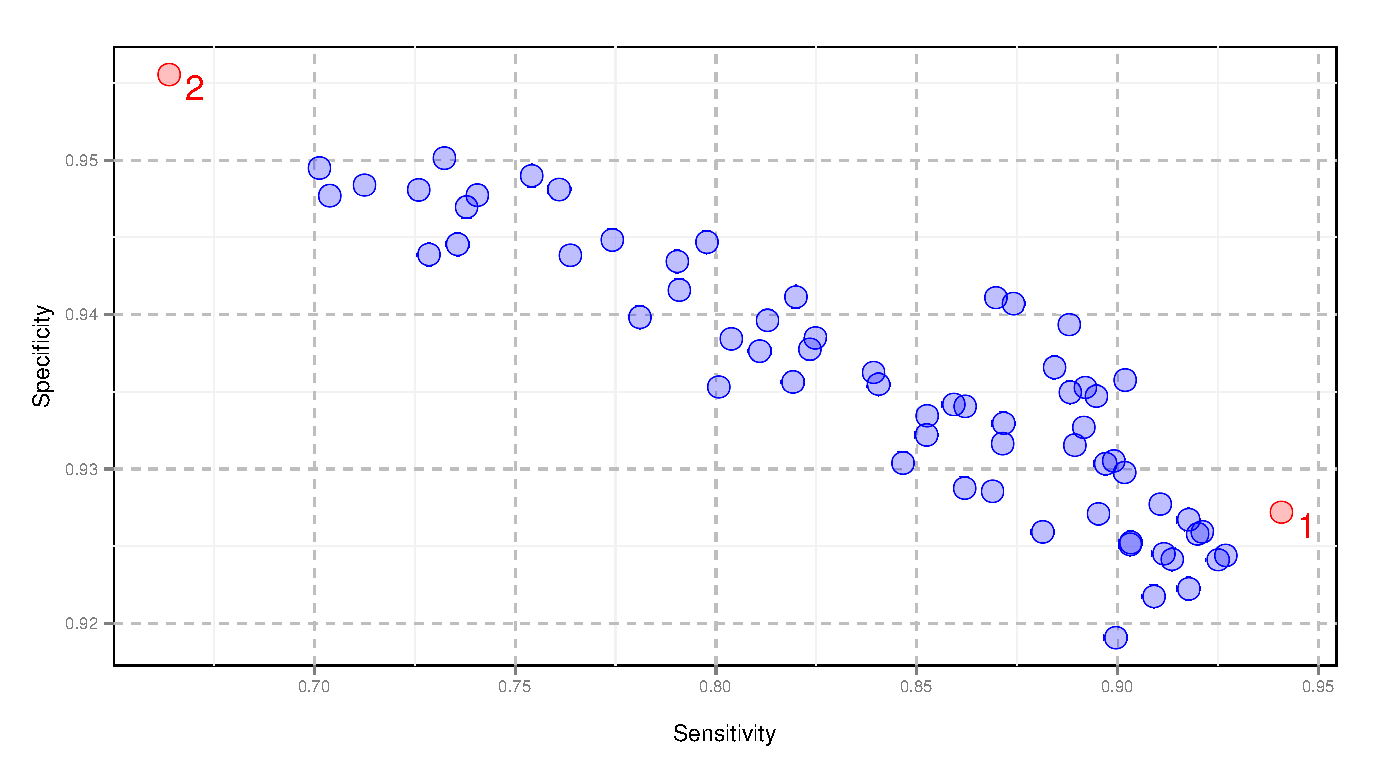
\includegraphics[width=0.95\textwidth, height=7cm]{figures/cvres.eps}
\caption{Sensitivity and specificity of amino acid encodings after cross-validation. 1 indicates the encoding providing the best sensitivity ($\textrm{AUC} = 0.9683$, $\textrm{MCC} = 0.8677$), whereas 2 means the encoding providing the best specificity ($\textrm{AUC} = 0.9338$, $\textrm{MCC} = 0.6474$). These encodings are shown in Tab.~\ref{tab:best} and Tab.~\ref{tab:worst}, respectively.}
\label{fig:cvres}
\end{figure}

\begin{table}[ht]
\begin{minipage}{.5\linewidth} 
\centering
\caption{The encoding of amino acids with the best sensitivity.} 
\begin{tabular}{ll}
  \toprule
Group & Amino acids \\ 
  \midrule
1 & D, E, H, K, N, Q, R \\ 
   \rowcolor[gray]{0.85}2 & G, P, S, T, Y \\ 
  3 & F, I, L, M, V, W \\ 
   \rowcolor[gray]{0.85} 4 & A, C \\ 
   \bottomrule
\end{tabular}
\label{tab:best}
%\end{table}

\end{minipage}
\begin{minipage}{.5\linewidth}
%\begin{table}[ht] 
\centering
\caption{The encoding of amino acids with the best specificity.} 
\begin{tabular}{ll}
  \toprule
Group & Amino acids\\ 
  \midrule
1 & A, E, K, Q, R\\ 
   \rowcolor[gray]{0.85} 2 & D, G, N, P, S, T\\ 
  3 & C, H, I, L, M, V\\ 
   \rowcolor[gray]{0.85} 4 & F, W, Y\\ 
   \bottomrule
\end{tabular}
\label{tab:worst}
\end{minipage}
\end{table}


\begin{figure}[ht]\centering
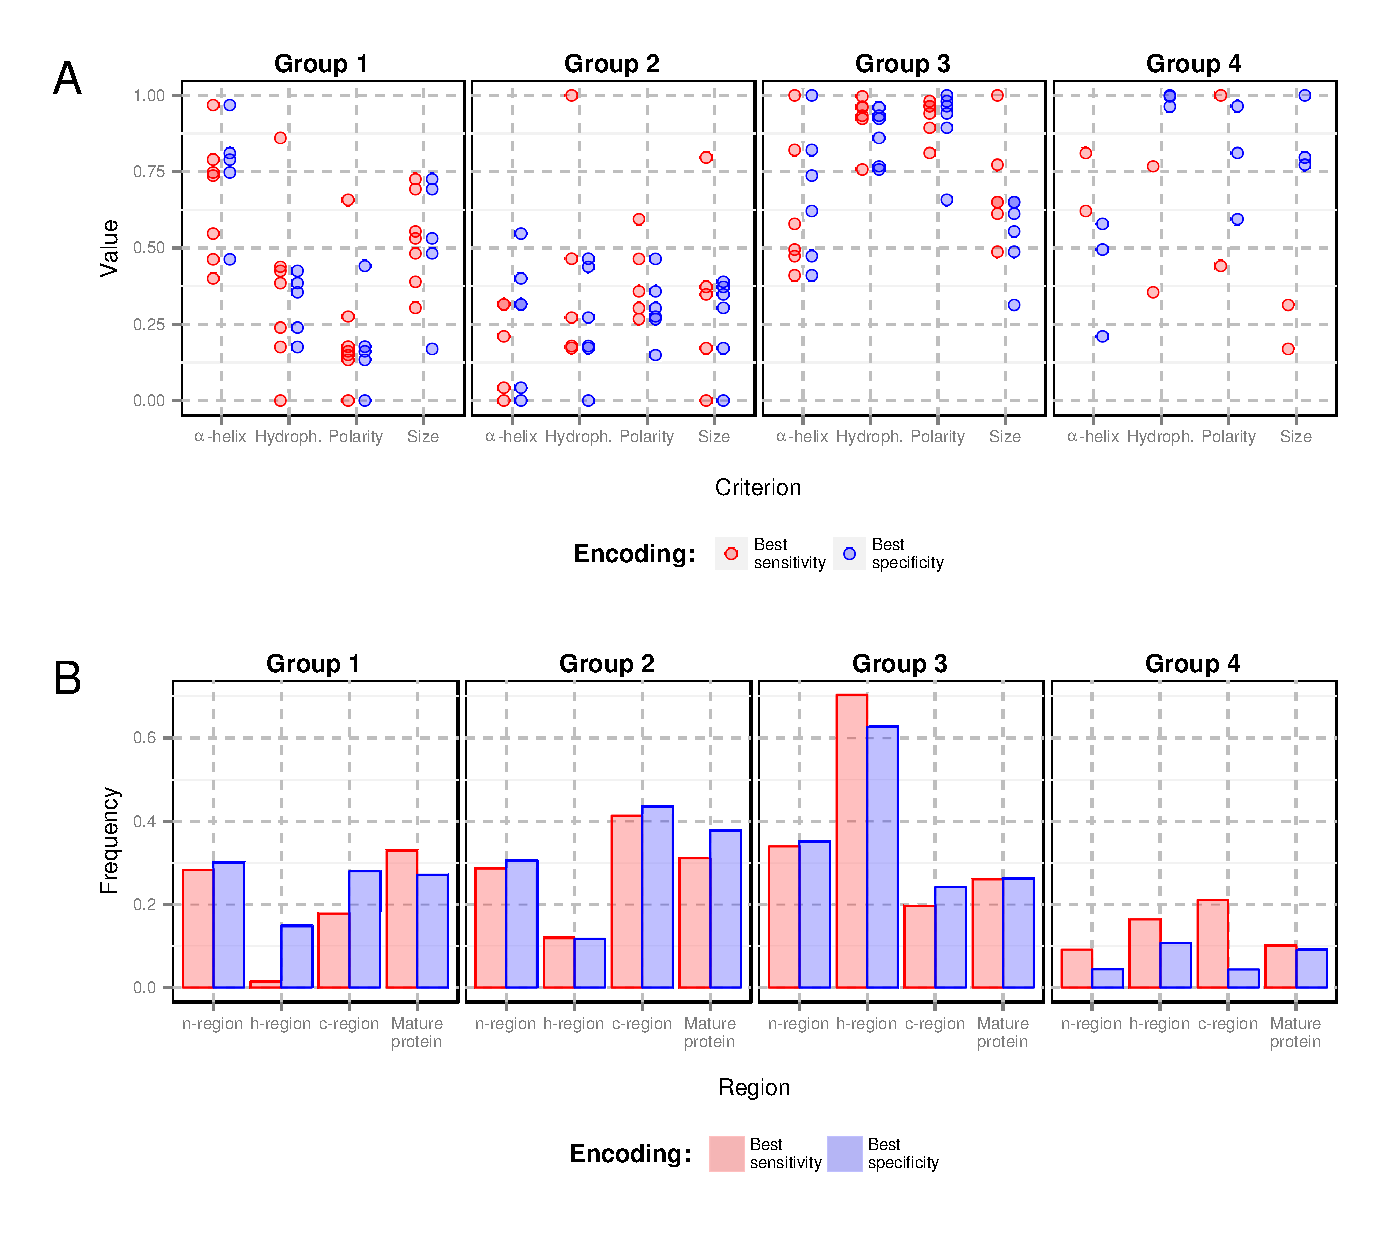
\includegraphics[width=0.95\textwidth]{figures/enccomp.eps}
\caption{Comparison of amino acid classified into four groups providing the best sensitivity and the best specificity in recognition of signal peptides. A. The normalized value of properties for particular amino acids represented by points. B. Frequencies of amino acids from the four groups in different regions of signal peptide and mature proteins.}
\label{fig:enccomp}
\end{figure}

To evaluate efficiency of our algorithm, we calculated four performance measures after cross-validation procedure for all amino acid encodings: specificity, sensitivity, Matthew's Correlation Coefficient ($\phi$ coefficient) and Area Under the Curve (AUC). The measures were characterized by very small variance (see for example Tab.~\ref{tab:perfmeas}), which indicates the credibility of the applied 5-fold cross-validation with 60 repetitions. All encodings of amino acids showed very good and quite narrow range of AUC (0.93 -- 0.97) and specificity (0.92 -- 0.96). However, sensitivity characterized by much wider variation and ranged from 0.66 to 0.94 (Fig.~\ref{fig:cvres}). For the final signalHsmm algorithm, we selected the encoding that yielded the highest sensitivity and the largest Matthew's Correlation coefficient as well as the second best AUC (Tab.~\ref{tab:best}).



\begin{table}[ht]
\centering
\caption{Performance measures for the amino aid encoding with the highest sensitivity calculated for 60 repetitions of cross-validation.} 
\label{tab:perfmeas}
\begin{tabular}{lrr}
  \toprule
Measure & Mean & SD \\ 
  \midrule
AUC & 0.9682 & 0.0023 \\ 
   \rowcolor[gray]{0.85}Sensitivity & 0.9407 & 0.0008 \\ 
  Specificity & 0.9272 & 0.0050 \\ 
   \rowcolor[gray]{0.85}MCC & 0.8681 & 0.0049 \\ 
   \bottomrule
\end{tabular}
\end{table}

\subsection*{Comparison of amino acid encodings}

We examined in detail composition of encodings and properties of their amino acids with the best sensitivity and the best specificity (Tab.~\ref{tab:best}, Tab.~\ref{tab:worst} and Fig.~\ref{fig:enccomp}). In both cases, the group 1 tends to contain generally average-sized polar amino acids. This group in the best sensitivity encoding is more uniform because it includes all charged amino acids, both acidic and basic (also weakly basic histidine), whereas in the best specificity encoding, it does not have histidine, aspartic acid and its amide but contains alanine. These amino acids are nearly absent from h-region and provide very good distinction between regions of signal peptide (Fig.~\ref{fig:enccomp}). In the best specificity encoding, where polar and charged character of the group 1 is not so explicit, the difference in its distribution between the regions is also less visible.

The amino acids belonging to the group 2 show generally a quite low probability of occurrence in $\alpha$-helix. The best sensitivity encoding comprises two types amino acids: all three hydroxylated residues as well as aliphatic glycine and proline known to break $\alpha$-helices. The best specificity encoding lacks tyrosine but includes in addition aspartic acid and its amide, which increase the polar character of this group. Despite these differences, the occurrence of the group 2 from both encodings is very similar in signal peptide's regions (Fig.~\ref{fig:enccomp}). This group is the rarest in h-region and the most frequent in c-region. 

Both encodings have strongly non-polar and aliphatic amino acids in group 3 such as: isoleucine, leucine, methionine and valine. The hydrophobic property of this group is  pronounced in the best sensitivity encoding by the presence of aromatic tryptophan and phenylalanine, whereas the group 3 in the best specificity encoding includes also hydrophobic cysteine and slightly basic but aromatic histidine. Because of the hydrophobic character, this group dominates in the h-region in the both amino acid classifications (Fig.~\ref{fig:enccomp}).

The fourth group is the most diverse in both encodings. In the case of the best sensitivity encoding, this group comprises only alanine and cysteine, which are rather small amino acids and tend to appear in $\alpha$-helices. This very unique composition seems to be the most typical to the c-region of signal peptide. In contrast, the group 4 in the best specificity encoding contains large aromatic amino acids: phenylalanine, tryptophan and tyrosine without special preference to signal peptide's regions.  

The encodings of amino acid plays crucial role in the recognition of signal peptide but does not affect in such extent identification of proteins without signal peptides. The change in specificity for different encodings is seven times smaller than for sensitivity (Fig.~\ref{fig:cvres}). It results from more uniform distribution of different residues in the part of mature protein than in signal peptide's regions.

\subsection*{Benchmark tests}

To provide the honest comparison of our algorithm with previous software, we trained our model on 2311 signal peptide-containing sequences deposited in Uniprot until 2010 year (the iteration of signalHsmm called signalHsmm-2010). The data set should correspond to the set used to train SignalP 4.1, the newest classifier present in the benchmark. In addition to this, we prepared the smaller data set, covering only 336 sequences collected till 1987 year, just after the first method predicting signal peptide was published~\cite{1986vonheijnea}. The signalHsmm-1987 iteration had to extract the signal peptide model from data set more limited than training sets of any classifier included in the benchmark.

Together with signalHsmm, we evaluated several signal peptide predicting algorithms in recognition of atypical signal peptides from malaria parasites: SignalP 4.1, PrediSi, Phobius and Philius (see Tab.~\ref{tab:bench2010plas} for the most common performance measures, and Supplemental Table~\ref{tab:bench2010plas_full} for 23 performance measures). The older version of SignalP 4.1, SignalP 3.0, was also incorporated in the analysis, because it is often chosen over its newer counterpart in the analysis of sequences belonging to Apicomplexa and other taxa due to the increased sensitivity ~\cite{2012cilingirapicoap, sperschneider_evaluation_2015}. 
Our algorithm obtained the greatest AUC, MCC and maximal sensitivity. For 12 of 23 performance measures, signalHsmm was the best or as good as others and for no parameter, it obtained the worst position (Supplemental Table~\ref{tab:bench2010plas_full}). PrediSi received the best specificity but at the expense of significantly reduced sensitivity.

We trained several iterations of signalHsmm  described above to check improvements introduced to our software: a new probabilistic model (hidden semi-Markov model) and a simplified alphabet of amino acids. The latter was compared with the version trained on raw amino acids sequences, denoted as 'raw aa' in Tab.~\ref{tab:bench2010plas}. The performance of this iteration was  worse than performance of its counterpart trained on the reduced alphabet. The version with the amino acid encodings outperformed the version with simple amino acids in 20 of 23 measures (Supplemental Table~\ref{tab:bench2010plas_full}). This result confirms that unique function of signal peptide does not depend on specific amino acids, but on more general features and our simpler model is able to recognize the unique architecture of signal peptide more accurately.

The advantage of hidden semi-Markov model over normal Markov model can be seen through the comparison of the signalHsmm with signal peptide predictors utilizing HMM: Phobius, Philius and SignalP 3.0 (HMM) - Tab.~\ref{tab:bench2010plas}. In all cases, the signalHsmm performed best for AUC and MCC. For the sensitivity, it obtained the largest value (1.0000) as SignalP 3.0. For 15 of 23 measures, our algorithm was best or as good as other software and never was the worst for any parameter (Supplemental Table~\ref{tab:bench2010plas_full}).

To check susceptibility of our model to overfitting, we trained several iterations on data sets with homology reduction 50\%. We discovered that our model, probably thanks to its relative simplicity, did not overfit and results were similar for models both with very restrictive and no homology reduction.

\begin{table}[ht]
\centering
\caption{Comparison of Area Under the Curve (AUC), H-measure and Matthews Correlation Coefficient (MCC) for different classifiers according to singal peptide-containing proteins from members of \textit{Plasmodiidae}. The abbreviations 'tm' and 'no tm' indicate version considering and not considering transmembrane domains, whereas 'hom. 50\%' means reduction of sequence homology for 50\% similarity.} 
\label{tab:bench2010plas}
\begin{tabular}{rllll}
  \toprule
 & Sensitivity & Specificity & MCC & AUC \\ 
  \midrule
signalP 4.1 (no tm) \cite{2011petersensignalp} & 0.8235 & 0.9100 & 0.6872 & 0.8667 \\ 
   \rowcolor[gray]{0.85}signalP 4.1 (tm) \cite{2011petersensignalp} & 0.6471 & 0.9431 & 0.6196 & 0.7951 \\ 
  signalP 3.0 (NN) \cite{2004bendtsenimproved} & 0.8824 & 0.9052 & 0.7220 & 0.8938 \\ 
   \rowcolor[gray]{0.85}signalP 3.0 (HMM) \cite{2004bendtsenimproved} & 0.6275 & 0.9194 & 0.5553 & 0.7734 \\ 
  PrediSi \cite{2004hillerpredisi} & 0.3333 & \textbf{0.9573} & 0.3849 & 0.6453 \\ 
   \rowcolor[gray]{0.85}Philius \cite{2008reynoldstransmembrane} & 0.6078 & 0.9336 & 0.5684 & 0.7707 \\ 
  Phobius \cite{2004klla} & 0.6471 & 0.9289 & 0.5895 & 0.7880 \\ 
   \rowcolor[gray]{0.85}signalHsmm-2010 & 0.9804 & 0.8720 & 0.7409 & 0.9262 \\ 
  signalHsmm-2010 (hom. 50\%) & \textbf{1.0000} & 0.8768 & \textbf{0.7621} & \textbf{0.9384} \\ 
   \rowcolor[gray]{0.85}signalHsmm-2010 (raw aa) & 0.9804 & 0.8720 & 0.7409 & 0.9262 \\ 
  signalHsmm-1987 & 0.9216 & 0.8910 & 0.7271 & 0.9063 \\ 
   \rowcolor[gray]{0.85}signalHsmm-1987 (hom. 50\%) & 0.9412 & 0.8768 & 0.7194 & 0.9090 \\ 
  signalHsmm-1987 (raw aa) & 0.9216 & 0.8863 & 0.7196 & 0.9039 \\ 
   \bottomrule
\end{tabular}
\end{table}

The overall simplicity of our approach does not hinder its capabilities of recognizing signal peptides from other taxa. We also benchmarked signalHsmm iterations and other software on the set of 127 eukaryotic proteins with signal peptide added after year 2010 to UniProt and randomly chosen 127 proteins without signal peptide. Their homology in the testing set was also reduced as described above. SignalHsmm-2010 performed comparably to SignalP 4.1. Both achieved AUC above 0.97 (see Supplemental Table~\ref{tab:bench2010_full} for all performance measures). Our algorithm was the best in AUCH and never obtained the worst note in comparison to seven programs. For eight measures it was the second in the ranking.

\subsection*{Conclusions}

We proposed a novel solution to the problem of predicting signal peptides, which appeared very efficient in recognition of atypical signal peptides from proteins of \textit{Plasmodiidae} although the program was trained on data coming from all eukaryotes. It indicates that our algorithm is able to describe common features of all signal peptides basing on the classical division of signal peptide into three regions. Our software is not limited to very specific taxonomic group, but is able to compete with state-of-art algorithms in predicting signal peptides of other organisms.

One of the most important features of signalHsmm is its stability. The difference in performance measures for versions trained on large and small data set deposited in databases in different times is negligible. It implies that signalHsmm extracts roughly the same general architecture of signal peptide regardless of the size and type of training data set. Similarly, iterations trained on data sets with and without removal of redundancy resulting from sequences homology showed the same prediction efficiency. It suggests that our probabilistic model is quite resistant to overfitting and does not adjust itself to most common patterns in training data sets but retrieves the universal model of signal peptide.

The existing software detecting signal peptides does not usually reveal decision rules responsible for this prediction. Our algorithm is the first step to explicitly show features of signal peptides important in their recognition, which is interesting from the biological point of view. The applied encoding of amino acids not only reduces the dimensionality of the problem, but also makes our probabilistic model more interpretable. Thanks to that, we were able to determine physicochemical properties of amino acids for particular regions of signal peptide. The model confirmed not only the high hydrophobicity of the h-region and polarity of the n-region but also found that hydroxylated amino acids are one of the most typical amino acids in the c-region. In contrast to the h-region, it also contains  $\alpha$-helix breakers: glycine and proline.

The flexibility and efficiency in recovery information make our model unique among similar software. SignalHsmm models properly very specific signal peptides belonging to narrow taxonomic groups which are poorly represented in databases and can effectively extract information from very small data sets. Our apporach may lead in future to development of new predictors specialized in recognition of atypical signals targeting sequences to subcellular compartments.


\subsection*{Availability and implementation}
The signalHsmm prediction web-server is available at: \url{http://smorfland.uni.wroc.pl/signalhsmm}. SignalHsmm is implemented as an R package available at: \url{http://cran.r-project.org/web/packages/signalHsmm}. Stand-alone version offers prediction and tools to build, train and test novel signal peptide models.

\section*{Supporting Information}

\beginsupplement
\subsection{Table}
\label{tab:bench2010plas_full}
{\bf Benchmark results - \textit{Plasmodiidae}.} Performance measures for benchmark test of signal peptide predictors using sequences belonging to \textit{Plasmodiidae}.

\subsection{Table}
\label{tab:bench2010_full}
{\bf Benchmark results - Eukaryots} Performance measures for benchmark test of signal peptide predictors using all eukaryotic sequences.


\section*{Acknowledgments}

\section*{Author Contributions}
MB and PM designed the study. All authors participated in the design of the study. PB and PS created the probabilistic model. MB and PS implemented the model and wrote the software. MB and PM wrote the manuscript. All authors critically revised the manuscript.

\nolinenumbers

\section*{References}

\bibliography{lokalizom}

% Either type in your references using
% \begin{thebibliography}{}
% \bibitem{}
% Text
% \end{thebibliography}
%
% OR
%
% Compile your BiBTeX database using our plos2015.bst
% style file and paste the contents of your .bbl file
% here.
% 
% \begin{thebibliography}{10}
% \bibitem{bib1}
% Devaraju P, Gulati R, Antony PT, Mithun CB, Negi VS. Susceptibility to SLE in South Indian Tamils may be influenced by genetic selection pressure on TLR2 and TLR9 genes. Mol Immunol. 2014 Nov 22. pii: S0161-5890(14)00313-7. doi: 10.1016/j.molimm.2014.11.005
% 
% \bibitem{bib2}
% Huynen MMTE, Martens P, Hilderlink HBM. The health impacts of globalisation: a conceptual framework. Global Health. 2005;1: 14. Available: http://www.globalizationandhealth.com/content/1/1/14.
% 
% \end{thebibliography}



\end{document}

